\section{GPU Results}
\label{sec:gpu-result}

In this section, we present the evaluation results of 44 benchmarks conducted successfully on our GPU node. Figure~\ref{fig:heatmap_gpu} illustrates the performance comparison between DaCe and NumPy running on a single-node CPU. Notably, our experimental environment employs a more recent version of DaCe compared to the one referenced in the original work~\cite{dace2021}, enabling the execution of additional benchmarks on the GPU platform. 
The majority of our findings align with those reported in the original work~\cite{dace2021}. For instance, benchmarks like \texttt{cholesky} and \texttt{ludcmp} exhibit slower performance on the GPU, while \texttt{clipping} and \texttt{heat3d} continue to demonstrate significant speedups of over 100x compared to NumPy. On the other hand, it is also important to note that the additional atomic operations introduced in \texttt{resnet} cause DaCe to perform more slowly on the GPU compared to NumPy. This issue is consistent with our observations in Section~\ref{sec:cpu-result} and is also documented in the original work~\cite{dace2021}.
% The majority of the results align with those presented in the original work~\cite{dace2021}. For example, \texttt{cholesky} and \texttt{ludcmp} exhibit slower performance on the GPU, while \texttt{clipping} and \texttt{heat3d} continue to demonstrate significant speedups of over 100x compared to NumPy. On the other hand, the additional atomic operations introduced in resnet also makes DaCe running on GPU performs slower comparing to NumPy. Such issue is also observed in Section~\ref{sec:cpu-result} and in the authors work~\cite{dace2021}.

\begin{figure}[!tp]
    \centering
    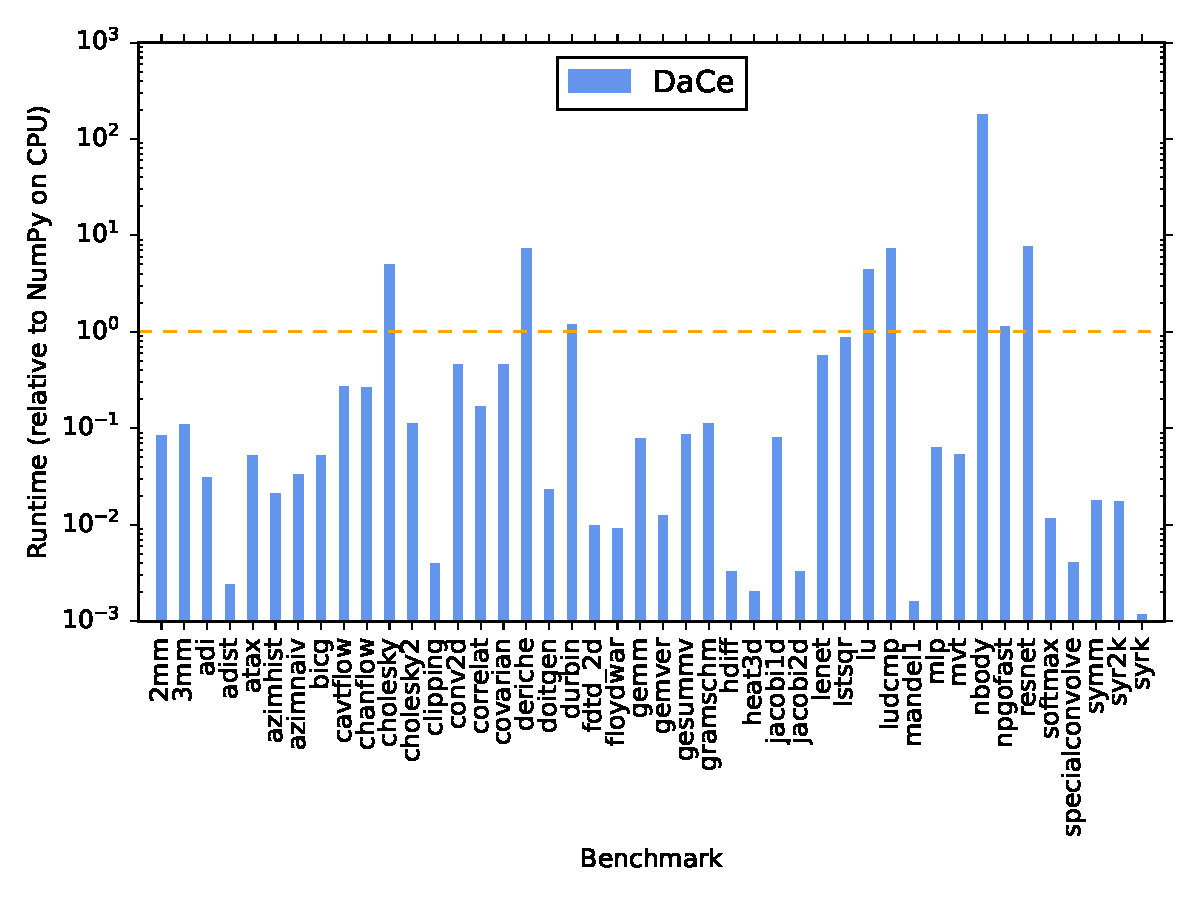
\includegraphics[width=.45\textwidth]{imgs/heatmap_gpu.pdf}
    \caption{DaCe GPU runtime normalized to NumPy on CPU (lower is better).}
    \label{fig:heatmap_gpu}
\end{figure}

In addition to observing similar results, we selected several benchmarks that exhibited either speedup or performance degradation to provide further analysis. Specifically, we analyze \texttt{cholesky}, \texttt{ludcmp}, \texttt{adist}, and \texttt{cholesky2}. The first two benchmarks demonstrate slower performance on the GPU, while the latter two show improved performance.

The reason behind the poorer performance of \texttt{cholesky} and \texttt{ludcmp} on the GPU is the communication and synchronization time between the CPU and GPU, which acts as a bottleneck. These benchmarks involve numerous scalar operations nested inside loops that cannot be parallelized. Since each scalar operation must be executed by a GPU kernel, significant communication overhead is introduced. Additionally, the problem size of each GPU kernel function is too small to effectively hide the communication overhead through computation.

The benchmark \texttt{cholesky2} implements the same algorithm as \texttt{cholesky}, but it invokes the NumPy linear algebra function. DaCe recognizes this and ports it to the GPU by utilizing cuBLAS~\cite{cublas}, the CUDA implementation of the Basic Linear Algebra Subprograms (BLAS) library. This optimization significantly improves the performance on the GPU.

Regarding the \texttt{adist} benchmark, we discovered that NumPy is unable to leverage Intel MKL and parallel processing for mathematical functions on arrays (e.g., \texttt{np.sin()})~\cite{numpy_pp}. However, DaCe is capable of exploiting data parallelism and dispatching computations on the GPU, leading to improved performance in this scenario.